\documentclass[12pt]{article}

%%%\usepackage{lucbr,graphicx,fancyhdr,longtable}
%\usepackage{lucidabr,graphicx,fancyhdr,longtable}
\usepackage{graphicx,fancyhdr,longtable}

\newcommand{\kc}{\textsf{kCARTA}\xspace}
\newcommand{\kl}{\textsf{kLAYERS}\xspace}
\newcommand{\cm}{\hbox{cm}}

% make a single, doubly indented line 
% (mainly used for driver file examples)
\newcommand{\ttab}{\indent\indent}

\input ASL_defs

\setlength{\textheight}{7.5in}
\setlength{\topmargin}{0.25in}
\setlength{\oddsidemargin}{.375in}
\setlength{\evensidemargin}{.375in}
\setlength{\textwidth}{5.75in}

\newlength{\colwidth}
\setlength{\colwidth}{8cm}
\newlength{\colwidthshort}
\setlength{\colwidthshort}{6cm}

\definecolor{light}{gray}{0.75}

\pagestyle{fancy}

% \date{July 5, 1994} % if you want a hardcoded date

\lhead{\textbf{\textsf{DRAFT}}}
\chead{kCARTA}
\rhead{\textsf{Version 1.0}}
\lfoot{UMBC}
\cfoot{}
\rfoot{\thepage}

\newcommand{\HRule}{\rule{\linewidth}{1mm}}
\newcommand{\HRulethin}{\rule{\linewidth}{0.5mm}}

\begin{document}
\thispagestyle{empty}
\vspace{2.0in}

\noindent\HRule
\begin{center}
\Huge \textbf{\textsf{kCARTA}}: An Atmospheric Radiative Transfer Algorithm 
using Compressed Lookup Tables
\end{center}
\noindent\HRule

\vspace{0.75in}
\begin{center}
\begin{Large}
Sergio De Souza-Machado, L. Larrabee Strow,\\ Howard Motteler and Scott
Hannon
\end{Large}
\end{center}

\vspace{0.5in}
\begin{center}
Physics Department\\
University of Maryland Baltimore County\\Baltimore, MD 21250 USA\\
\end{center}

\vspace{0.5in}
\begin{center}
Copyright 2011 \\
University of Maryland Baltimore County \\
All Rights Reserved\\
v1.00  \today\\
\end{center}

\vfill

\noindent\HRulethin
\begin{flushleft}
\begin{tabbing}
Sergio~De~Souza-Machado: \=    sergio@umbc.edu \\
L.~Larrabee~Strow:   \>        strow@umbc.edu\\
\end{tabbing}
\end{flushleft}

%\begin{flushright}
%\includegraphics[width=1.0in]{umseal.eps}
%\end{flushright}

\newpage
\tableofcontents
%\listoftables
%\listoffigures
\newpage

\begin{center}
{\bf ABSTRACT}
\end{center}
\kc is a radiative transfer code for a non-scattering Earth's
atmosphere.  As packaged, it can be used to output monochromatic gas optical
depths, and clear sky radiances and jacobians. This Matlab package is a 
simpler version of the f77 version, which includes scattering and fluxes.

The code is driver by profiles in the .rtp format allowing the user to easily 
change atmospheric conditions as needed. US Standard Atmosphere optical 
depths have been precomputed and saved to a lookup table. This means (linear)
interpolations required to compute the optical depths for arbitrary atmospheric
profiles can be done very rapidly, as can the derivatives needed for 
the Jacobians. This makes \kc very fast. 

The code in the basic Test package allows the user to do RT calculations for 
a downlooking instruments at the top of atmosphere (TOA), as well as code to 
only compute optical depths. This basic package assumes the "klayers" levels
are the same as those in the kCompressed Database. NLTE radiance effects in the
4 um CO2 band are included in daytime RT calculations.

A more versatile package allows one to to use pressure layerings different
than that of the kCompressed Database. This is required for uplooking 
instruments as the rapid variation of temperature and profile gas constituents
near the instrument, require a finer layering than that of the standard
kCompressed pressure layering. 

We hope that the ease of use, range of features and speed of \kc, make it a 
useful tool. In addition to the main \kc source code, some packages need to be 
picked up. One is \kl, which allows an user to input a radiosonde or 
model point profile, and output a layer averaged profile that \kc can use. 
Another is the $RTP$ package, which is a AIRS Level II file format. 

This document is very much a work in progress.  Some major omissions
include references, significant examples of \kc output, and
comparisons of \kc output to observed spectra.  These omissions will
be rectified in the future.  Please give us your feedback on both the
code and the documentation!

\newpage
\section{Introduction}

\kc stands for ``kCompressed Atmospheric Radiative Transfer
Algorithm.''  This is an infrared, ``monochromatic'' radiative
transfer algorithm written for a one dimensional non-scattering Earth
atmosphere. 

At the heart of the code are routines to uncompress an optical depth database,
computed for the US Standard Profile and for 10 temperature offsets 
(-50 K, -40K, ..., +40 K, +50 K) from this profile. This makes computing 
optical depths for any realistic Earth atmosphere very fast and accurate, as 
the code only needs to interpolate the arbitrary profile using this underlying
temperature grid. Uncompressing the database also rapidly yields analytic 
temperature jacobians. 

The code was originally written in F77, and morphed to include upwelling and
downwelling clear sky radiative transfer calculations, calculations in a 
scattering atmosphere, NLTE effects in the 4 um CO2 band, and fluxes and
heating rates calculations. This Matlab package encapsulates the uncompression
routines, and provides examples of how to produce clear sky optical depths 
and radiative transfer calculations. The package is tied in with UMBC 
\kl and "RTP" packages. The former takes a levels profile, and produces 
a layers averaged profile. The latter is a .hdf based file format, and allows 
us to include all necessary parameters (such as profile information, satellite
and solar angles, emissivities) into a "Radiative Transfer Protocol" file.

\section{Radiative transfer}
For a downward looking instrument, in a clear sky, 
the surface term and layer emission terms are automatically included in the 
radiative transfer calculation.  In addition, reflected thermal and solar 
terms can also be included  :
\begin{equation}
R(\nu) = R_{\hbox{\it surface}}(\nu) + R_{\hbox{\it layer emission}}(\nu) + 
R_{\hbox{\it thermal}}(\nu) + R_{\hbox{\it solar}}(\nu)
\end{equation}
where the terms are the surface, layer emissions, reflected thermal
and solar respectively.  The reflected thermal term is computed
accurately by determining (monochromatically) the layer to ground
cumulative sum of absorption coefficients, and then using an optimum
diffusive angle based on a parameterization of angle as a function of
this cumulative sum.  This makes the inclusion of reflected thermal in
the code quick and accurate.   By differentiating the radiance equation
with respect to a layer gas amount or temperature, the radiance
Jacobian is obtained.  Dropping the surface and reflected thermal terms
enables \kc to compute the radiance measured by an upward looking
instrument as well. The radiative transfer routines include effects of
curvature on angles that deviate from nadir.

More documentation on the driver files, and on the convolution routines, 
can be found in the appropriately named pdf files.

\section{Analytic Jacobians}
Taking into account the view angle correction, if $\tau_{i}$ is the optical 
depth due to gas G at layer $i$, given by $\tau_{i} = q_{i} K_{i}/\mu{i}$ 
where the symbols respectively stand for optical depth (dimensionless), gas 
amount (kmoles/cm2), gas absorption (cm2/kmol) and $cos(view angle)$, then 
the finite difference column gas jacobian is 
given by the difference between the new and unperturbed radiances 
$\delta r$ = $r_{new} - r-{0}$ when the gas amounts in layers $1$ to $N$ are 
perturbed by a fraction $\delta$. The (finite differences) column jacobians 
can be obtained from the (gas) layer analytic jacobians using
\[
\delta r = \frac{\partial r}{\partial q_1} \delta q_1 + 
           \frac{\partial r}{\partial q_2} \delta q_2 + ... + 
           \frac{\partial r}{\partial q_N} \delta q_N
\] 
or 
\[
\delta r = J_{1} \delta q_1 + J_{2} \delta q_2 + ...
               J_{N} \delta q_N
\]
Usually we take a constant perturbation to the column ie $q_{l} \rightarrow 
q_{1}(1 + f)$ where $f \ll 1$. Then $\delta q_{l} \rightarrow f q_{l}$ and
$\delta r = f \{ J_{1} q_1 + J_{2} q_2 + ... + J_{N} q_N \} $. For example, 
for a 2 layer atmosphere the upwelling radiance (without background thermal 
or solar terms)jacobian terms $J_{l}$ is 
\begin{eqnarray*}
r = & \epsilon B(T_{s}) exp(-q_{1} K_{1}/\mu_{1})exp(-q_{2} K_{2}/\mu_{2}) +\\
    & B(1)(1-exp(-q_{1} K_{1}/\mu_{1}))exp(-q_{2} K_{2}/\mu_{2}) + \\
    & B(2)(1-exp(-q_{2} K_{2}/\mu_{2}))
\end{eqnarray*}
from which the layer jacobian terms $J_{i}$ reduce to
\begin{eqnarray*}
J_{1} = \frac{\partial r}{\partial q_1} = & 
 -\frac{K_1}{\mu_1}\epsilon B(T_{s})exp(-q_1 K_1/\mu_1)exp(-q_2 K_2/\mu_2) + \\
&-\frac{K_1}{\mu_1} B(1)(exp(-q_{1} K_{1}/\mu{1})exp(-q_{2} K_{2}/\mu{2})
\end{eqnarray*}
\begin{eqnarray*}
J_{2} = \frac{\partial r}{\partial q_2} = & 
-\frac{K_2}{\mu_2}\epsilon B(T_{s})exp(-q_1 K_1/\mu_1)exp(-q_2 K_2/\mu_2) + \\
& -\frac{K_2}{\mu_2} B(1)exp(-q_{1} K_{1}/\mu{1})exp(-q_{2} K_{2}/\mu{2}) + \\
& -\frac{K_2}{\mu_2} B(2)exp(-q_{2} K_{2}/\mu{2})
\end{eqnarray*}

\section{kCompressed Database}

Optical depths are computed for all molecules in the HITRAN database, using
a profile derived from the 1962 US Standard Atmosphere. These optical
depths are pre-computed using a Matlab based line by line code.

The current database spans 605 \wn to 2805 \wn, broken up into chunks
that are 25 \wn wide. The point spacing of the current database is 0.0025 \wn,
which is an average over five points spaced at 0.0005 \wn.
One hundred pressure layers are used to generate the 
database, from 1100 mb down to 0.005 mb.  These pressure layers are the same 
as those used for the AIRS (Atmospheric InfraRed Sounder) Fast Forward Model, 
for which \kc is the ``Reference Forward Model.''The thickness of the layers 
is roughly 250 m close to the surface, gradually increasing to as much as 
2000m in the upper atmosphere. The 100 layers were carefully chosen so as to 
keep errors at the 0.1 K level, comparable to noise levels in contemporary 
sounders.

The temperatures in the spectroscopic database are computed at the Standard 
Profile, as well as ten temperature offsets (in increments of $\pm$ 10K) on 
either side of the Standard Profile. These optical depth tables are compressed
using a Singular Value Decomposition ({\sf SVD}) technique, to produce our 
{\sf kCompressed} database.  

The current spectroscopic compressed
tables use the {\sf HITRAN98} database for both line-parameters and
cross-sections.  The full and first-order $CO_{2}$ linemixing is from 
refining the modeling undertaken by David Tobin. It should be more accurate 
than that currently in {\sf GENLN2}. in addition, we have used the latest
O2 and N2 continuum models (see Lafferty and J.-M. Hartmann et al in Applied 
Optics 1996, 1997). Other updates to spectroscopy include the ``local'' 
water lineshape as defined by CKD.

To compute the absorption coefficients for an arbitrary profile, the look-up 
tables are interpolated in temperature, and scaled in gas absorber amount.  
These interpolations allow easy computation of analytic temperature 
derivatives, from which we can compute temperature Jacobians. \kc is not 
limited to these 100 AIRS pressure levels/layers. The user can change the 
pressure levels scheme in \kl, and \kc will then also do a pressure 
interpolation (as long as the new pressures span 1100 to 0.005 mb). 

The speed and features of the code make it an appealing alternative to other
existing ``line by line'' codes such as {\sf GENLN2} and {\sf LBLRTM}.
The accuracy of the database has been extensively compared to {\sf
  GENLN2}.  \kc should contain the latest spectroscopy/lineshape information. 
The transmittances computed by \kc are smooth and well behaved, which 
will allow people to develop fast-forward models.

\section{GasIDs}
The gasIDs used by \kc and \kl follow the HITRAN convention. "gasids\_H2008" 
(and the earlier "gasids\_H92\_H2k") in this $DOC$ subdirectory, provide a list
of gasID vs commonly used name and/or chemical formula.

\section{Units and Definitions}

Frequencies are in units of wavenumbers (\wn), temperatures are in Kelvins. 
The gas profiles expected by \kc use path averages over the layers, and are 
in units of $\hbox{\em molecules} \cm^{-2}$.  Temperatures should be
specified in {\em kelvin}, while pressures and partial pressures
should be expressed in {\em millibar}. 

Output gas and mixed path optical depths are dimensionless (absorption
coefficient $\times$ gas amount); obviously so are transmittances.
Output radiances are in blackbody radiance units ($\hbox{\em milliwatts}
\;\ m^{-2} sr^{-1}/\cm^{-1}$).  Jacobians can be output in one of three
modes : (a) $d(\hbox{\em rad})/ds_{m}$, where $s_{m}$ is the temperature or 
gas amount in layer $m$, (b) $d(\hbox{\em rad})/ds_{m} \times Z_{m}$, 
where $s_{m}$ is the temperature or gas amount in layer $m$, and $Z_{m}$ is 
an unit perturbation (+1 K if temperature, or +gas amount in $m$th layer) and
(c) $d(\hbox{\em BT})/ds_{m} \times Z_{m}$, where $s_{m}$ is the temperature 
or gas amount in layer $m$, and $Z_{m}$ is an unit perturbation (+1 K if 
temperature, or +gas amount in $m$th layer)

\section{Installing and running \kc}
This is for the user that wants to install and use \kc as quickly as possible. 
We purposely keep this user manual short, and ask the user to 
examine the "user\_set*.m" codes in the \textcolor{blue}{Test} subdirectory 
in great detail, so as to understand how to use the package. 

\subsection{Distributing \kc}
The distribution is divided into three parts :

\begin{itemize}
\item \textcolor{blue} {Main tarfile $kcmix_matlabVYYY.tar$} where $YYY$ is 
the version number. This will contain the entire source code distribution, 
many needed data files, and the documentation. \\
\item \textcolor{blue} {kCompressed Database} : about 600Mb, supplied on CDs. 
We supply two versions, the big endian or the little endian versions \\
\end{itemize}

\subsection{Installing \kc}
Having obtained the above three, the user can now proceed to install \kc : 
\textcolor{blue} {Untar $kcmix_matlabVYYY.tar$} :  this will create a 
main subdirectory, named PACKAGE\_UPnDOWNLOOK\_2011, as well as many 
subdirectories containing the source code, data files and so on.

\begin{verbatim}
drwxr-xr-x 2 sergio pi_strow    7 Mar 24 17:31 Test
drwxr-xr-x 2 sergio pi_strow    4 Mar 24 17:29 RTPFILES
drwxr-xr-x 2 sergio pi_strow   13 Mar 24 17:23 DOC
drwxr-xr-x 2 sergio pi_strow   12 Mar 24 15:24 CONVOLUTION
drwxr-xr-x 6 sergio pi_strow   26 Mar 24 04:49 VariablePressure
drwxr-xr-x 6 sergio pi_strow    9 Mar 23 12:40 private
drwxr-xr-x 3 sergio pi_strow    4 Mar 23 10:35 JACDOWN
drwxr-xr-x 6 sergio pi_strow    6 Mar 22 15:38 DATA
\end{verbatim}

\section{Files in directories}

\subsection{Main directory \textcolor{red}{Usual 100 AIRS layers}}
This contains the main files a user should need \textcolor{red}{for a 
pressure layering that is the same as the AIRS 100 layers.} 

Routines for uncompressing
the database ($kcmix*.m$) and the continuum files ($cont*.m$), for doing
radiative transfer ($rtchunk\_Tsurf*.m$) are included here. The $\_nojac$ 
extension to the name means the faster (non jacobian version), while $\_jac$ 
is the slower, jacobian version. The main routines are 
$matlab\_kcarta\_downlook_*.m$

Note : if the user wants to edit which gases he/she should be included in the
"atmosphere", then look for the line that says "edit this list to only keep 
gases you DO want" in matlab\_kcarta\_downlook\_jac.m or 
matlab\_kcarta\_downlook\_nojac.m or matlab\_kcarta\_opticaldepths.m; 
default is to add $ALL$ gases.

\begin{verbatim}
auxiliary_set.m
contcalc2.m
contcalc2_S_F.m
continuum_temp_interp_weights_jac.m
continuum_temp_interp_weights.m
contjaccalc2.m
dirname.m
doload.m
find_chunks.m
initialize_extra.m
initialize_kcmix.m
kcmix2jac.m
kcmix2.m
matlab_kcarta_downlook_jac.m
matlab_kcarta_downlook_nojac.m
matlab_kcarta_opticaldepths.m
nlte.m
op_rtp_to_lbl2.m
rtchunk_Tsurf_jac.m
rtchunk_Tsurf.m
temp_interp_weights_jac.m
temp_interp_weights.m
\end{verbatim}

As given out, the code was optimized for the 605 - 2830 \wn spectral range which
is the range covered by AIRS, IASA, CRiS, and HIRS and AERI instruments. However
the code is flexible enough to allow optical depth and radiance calculations in
other spectral bands. Since the FWHM of lines gets smaller (larger) as the 
wavenumbers get smaller (larger), the resolution of the database must change.
Each file in each spectral range will contain 10000 points; so for example at the
default 0.0025 \wn resolution of the main IR default band (605-2830 \wn), the
files each span 25 \wn. We envisage the following :

\begin{verbatim}
  kcartachunks = 00080 : 0002.5 : 00150;  prefix = '/j';
  kcartachunks = 00140 : 0005.0 : 00310;  prefix = '/k';
  kcartachunks = 00300 : 0010.0 : 00510;  prefix = '/p';
  kcartachunks = 00500 : 0015.0 : 00605;  prefix = '/q';
  kcartachunks = 00605 : 0025.0 : 02830;  prefix = '/r'; ** default **
  kcartachunks = 02830 : 0025.0 : 03580;  prefix = '/s';
  kcartachunks = 03550 : 0100.0 : 05650;  prefix = '/m';
  kcartachunks = 05550 : 0150.0 : 08350;  prefix = '/n';
  kcartachunks = 08250 : 0250.0 : 12250;  prefix = '/o';
  kcartachunks = 12000 : 0500.0 : 25000;  prefix = '/v';
  kcartachunks = 25000 : 1000.0 : 44000;  prefix = '/u';
\end{verbatim}

\textcolor{red}{It is the responsibiliy of the user to set fA,fB in 
the "user\_set\_input*" files such that they only span $ONE$ spectral
range}. For example, one run covering 605-2830 \wn is fine, as is 
another run covering 500-605 \wn. But the code as written will not permit
a single run covering 500-2830 \wn.

\subsection{private}
This subdir contains files that are called by the main routines, and should
not be modified.

\subsection{DOC}
The documentation for this package

\subsection{CONVOLUTION}
Convolution routines. We include generic gaussian convolvers, as well as AIRS
SRF convolvers, and IASI/CRiS convolvers. Note the files contained in this 
subdir will not be supported.

\subsection{JACDOWN}
This has the main driver for a downlook jacobian calculation, "jac\_downlook.m"
which calls files in the $private$ subdirectory underneath this. One can speed
up the jacobian code by eg removing the looping over the weighting functions, 
or over the temperatures.

\subsection{RTPFILES}
Sample rtpfiles for this package; "desert" is a downlooking case at 100 AIRS
layers, while the other is an uplooking case at a different layering scheme.
In addition we provide a subdirectory with some binary files output from
the f77 code.

\subsection{DATA}
Contains subdirectories with continuum, solar, NLTE and CO2 Chifunction 
datafiles.

\subsection{\textcolor{blue}{Test}}
Examples of two driverfiles, one which computes optical depths (based on a 
list the user supplies), and the other which computes radiances (and 
jacobians if asked). The user should carefully examine these files, as they
provide a working outline of how to use this package.

Basically, the user is allowed to set the 
following parameters : which HITRAN version to use, start/stop wavenumbers for
the calculations, whether or not to do Jacobians, what output units for the
Jacobians, what CKD version, and name of input rtp file.
\begin{verbatim}
user_set_input_downlook.m        parameters driving dokcarta_downlook.m
user_set_input_opticaldepths.m   parameters driving dokcarta_opticaldepths.m
\end{verbatim}

The user needs to supply paths to where the solar files, continuum files,
nlte files, klayers executables, optical depth database and reference profiles
are; this is controlled via $user\_set\_dirs.m$
\begin{verbatim}
user_set_dirs.m                  set up the paths to directories
\end{verbatim}

Finally the user can commence the computation, calling one or the other
of the routines named below (which call relevant files from above).
\begin{verbatim}
dokcarta_downlook.m              compute RT
dokcarta_opticaldepths.m         compute optical depths
\end{verbatim}

This subdir also includes two matlab files, containing radiances output
using H2004 and H2008.

\subsection{VariablePressure \textcolor{red}{Different pressure layers}}
This contains the main files a user should need \textcolor{red}{for a 
pressure layering different than the AIRS 100 layers.} This makes the code(s)
slower. The structure and content of the directories is the same as before 
$viz$

\begin{verbatim}
drwxr-xr-x 2 sergio pi_strow    10 Mar 24 04:49 Test
drwxr-xr-x 6 sergio pi_strow     8 Mar 23 11:58 private
drwxr-xr-x 3 sergio pi_strow     4 Mar 23 10:36 JACUP_VarPress
drwxr-xr-x 3 sergio pi_strow     4 Mar 23 10:35 JACDOWN_VarPress
\end{verbatim}

\noindent $Test$ has dokcarta\_downlook.m, dokcarta\_uplook.m (very similar to 
the "downlook" case) and dokcarta\_opticaldepths.m.\\

\noindent $JADOWN\_VarPress$ has jacobian routines for downlooking 
instruments\\

\noindent $JACUP\_VarPress$ has jacobian routines for uplooking instruments\\

\section{Comparisons against f77 and our code}
We have tested this code against the f77 \kc code and across the IR bands, 
have errors less than 0.05 K in brightness temperature. The speeds are also
very similar (roughly about 60 seconds on a 2.6 GHz processor for a full
radiative transfer calculation).

The $Test$ directory contains "matlab\_test\_desert\_0725\_2004.mat" which is 
a radiance computation coming from running the "dokcarta\_downlook.m" in that
directory.

\begin{figure}
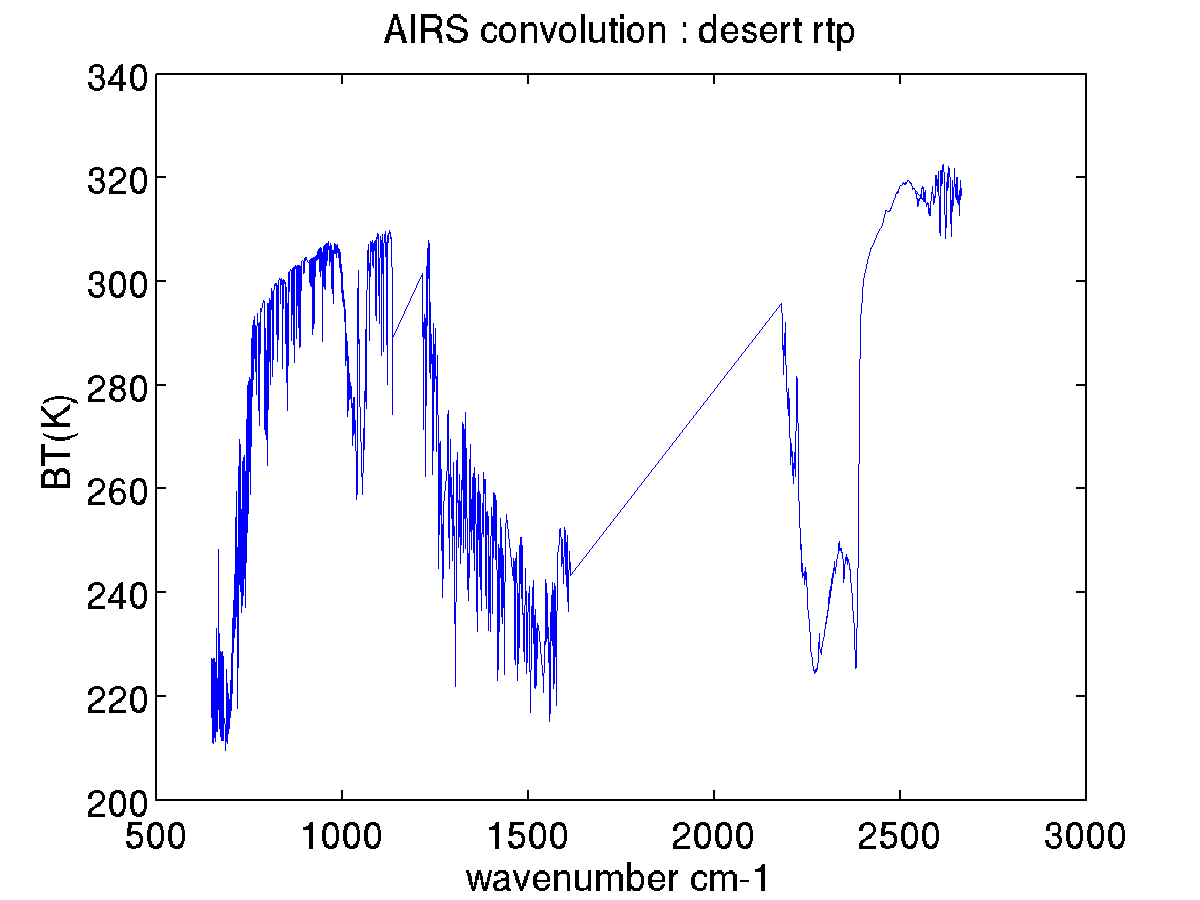
\includegraphics[width=5.5in]{desert_rtp.png}
\caption{Sample output from "desert\_op.rtp", convolved with AIRS SRFs}
\label{translatingfiles}
\end{figure}


\end{document}
